\documentclass[12pt]{article}

\usepackage{graphicx}
\usepackage{paralist}
\usepackage{amsfonts}
\usepackage{hyperref}
\usepackage{listings}
\usepackage{subfig}
\usepackage{float}

\oddsidemargin 0mm
\evensidemargin 0mm
\textwidth 160mm
\textheight 200mm
\renewcommand\baselinestretch{1.0}

\pagestyle {plain}
\pagenumbering{arabic}
\newcounter{stepnum}

\title{Course Project}
% \author{Hyosik Moon}
\author{
  Moon, Hyosik
  }

\begin {document}

\maketitle

\section{Required}

\begin{itemize}
\item \textbf{Main objective of the analysis} \\
We will optimize the `CartPole-v0' problem with three different models such as `RandomForestRegressor, AdaBoostRegressor, ExtraTreesRegressor'. The goal of the problem is to prevent a pole attached to a cart from falling over by increasing and reducing the cart's velocity. Whenever it successes to mainatain the pole, it gets a socre as a reward. We win the game, if we maintain the pole for 200 times.

\item \textbf{Brief description of the data set} \\
Because this is reinforcement problem we need to produce our own data set. In order to get the data set, I implemented the game 10000 times. We can check the data in the figure \ref{data}. Four observations represent `Cart Position', `Cart Velocity', `Pole Angle', and `Pole Angular velocity' respectively. 

\begin{figure}[H]
    \centering
    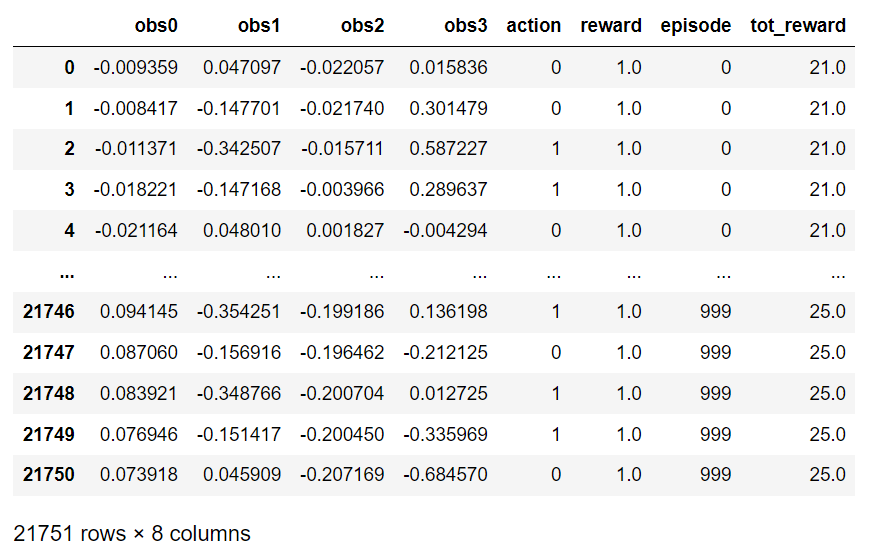
\includegraphics[width=0.9\textwidth]{figures/data.png}
    \caption{Data set information}\label{data}
\end{figure}

\item \textbf{Brief summary of data exploration}
In order to train a model, we need the pole's position, velocity, angle, angular velocity, and actions as x variable and reward as y value. So I made a dataframe and extract x and y from the dataframe in the figure \ref{data}.
    
    % \begin{figure}[H]
    %   \centering
    %   \subfloat[Correlation]{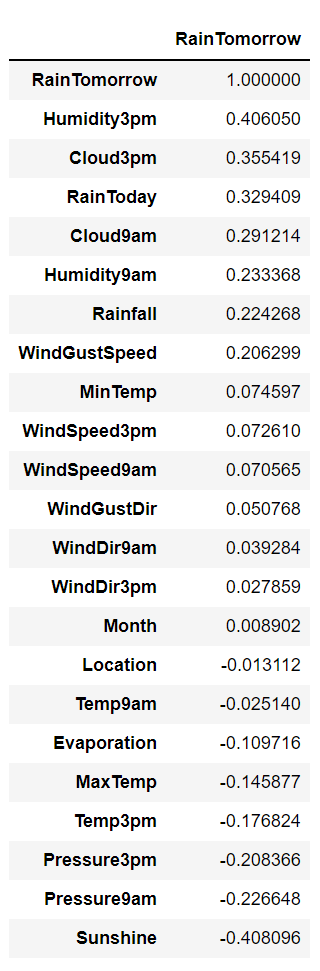
\includegraphics[width=0.3\textwidth]{figures/corr.png}\label{corr}}
    %   \hfill
    %   \subfloat[Correlation bar plot]{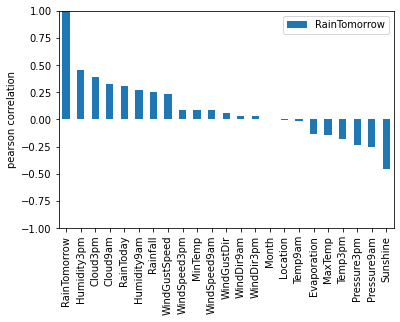
\includegraphics[width=0.65\textwidth]{figures/corr2.png}\label{corr2}}
    % \end{figure}

\item \textbf{Summary of training at least three models} I implemented the game with three different prediction models which are  `RandomForestRegressor, AdaBoostRegressor, and ExtraTreesRegressor'.
    \begin{enumerate}
      \item RandomForestRegressor. It showed the relatively good result. The average step maintaining the pole was 157, with a perfect score of 30 out of 100 trials. (Figure \ref{random_forest})
      \begin{figure}[H]
        \centering
        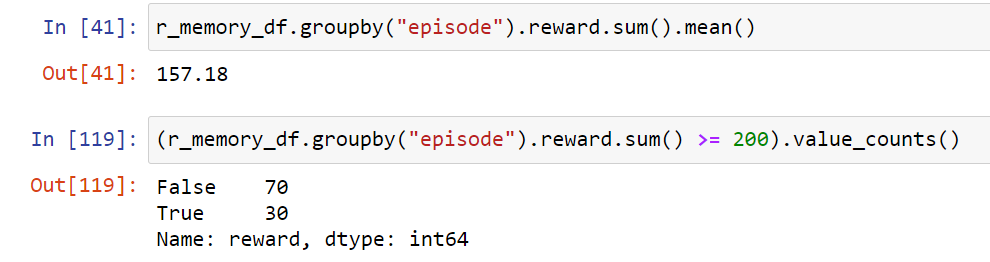
\includegraphics[width=0.9\textwidth]{figures/random_forest.png}
        \caption{Data set information}\label{random_forest}
      \end{figure}

      \item AdaBoostRegressor. The result was terrable. Because in the case of AdaBoost it modifies the weights sequencially with the wrongly predicted data set. Since our data set consists of randomly chosen episodes, the AdaBoost model might be inappropriate to train the this data. (Figure \ref{AdaBoost})
      \begin{figure}[H]
        \centering
        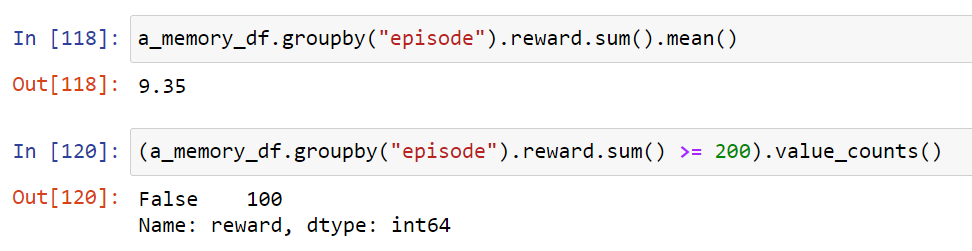
\includegraphics[width=0.9\textwidth]{figures/AdaBoost.png}
        \caption{Data set information}\label{AdaBoost}
      \end{figure}

      \item RandomForestRegressor. It showed the relatively good result. The average step maintaining the pole was 157, with a perfect score of 30 out of 100 trials. (Figure \ref{random_forest})
      \begin{figure}[H]
        \centering
        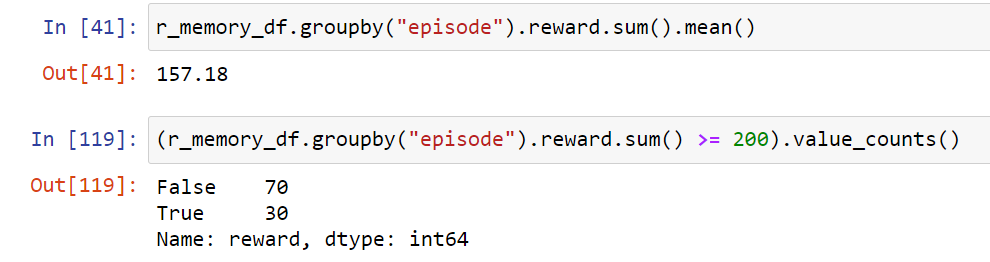
\includegraphics[width=0.9\textwidth]{figures/random_forest.png}
        \caption{Data set information}\label{random_forest}
      \end{figure}
    \end{enumerate}

\item \textbf{Explanation of your final model}
Overall, the RandomForestRegressor showed the best performance. I think that this is because we used closely related features to predict the result which are `Cart Position', `Cart Velocity', `Pole Angle', and `Pole Angular velocity'. Thus, the result of RandomForest is better than ExtraTreesRegressor because ETR models train the model with randomly chosen features. In order to increase the performance, I trained the final model (RandomForestRegressor) with more data which have 20000 trials. And the final result shows that the average step maintaining the pole was 161, with a perfect score of 28 out of 100 trials. (Figure \ref{rf})

\begin{figure}[H]
  \centering
  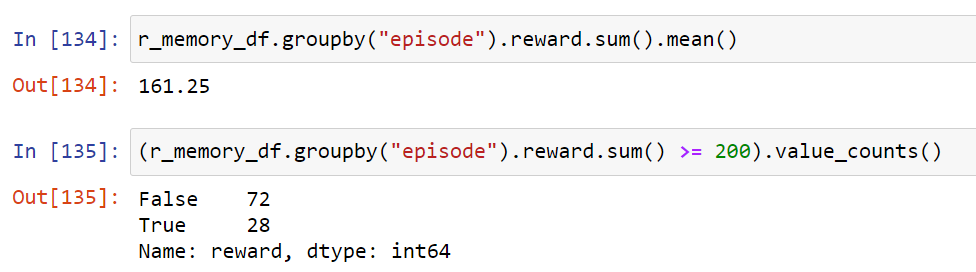
\includegraphics[width=0.9\textwidth]{figures/rf.png}
  \caption{Data set information}\label{rf}
\end{figure}

\item \textbf{Summary Key Findings and Insights}


\item \textbf{Suggestions for next steps}
In order to increase the success rate, using deep neural network can be another way. Thus I also made two neural networks models such as deep neural network, and recurrent neural network.

\end{itemize}

\end {document}